\documentclass{beamer}
\usepackage{graphicx} % includegraphics command is implemented here
\usepackage{spverbatim}
\usetheme{Hannover}
\author{Anton Saatze}
\title{Android LiveData}
\institute{University of applied Sciences Munich}
\date{22.may.2020}
\subject{Android}
\begin{document}
	\maketitle
	
	\begin{frame}
		\frametitle{Table of Contents}
		\tableofcontents
	\end{frame}
	
	\section[Motivation]{Motivation}
	\begin{frame}
		\frametitle{Motivation}
		\begin{itemize}
		\item core concept to present data
		\item clean way to hand data across the archictecture
		\item guarantee that latest data is presented in view
		\item first thing to learn, when joining a real android project team
		\end{itemize}
	\end{frame}
	
	\section[Technical Background]{Technical Background}
	\begin{frame}
		\frametitle{Technical Background}
		\begin{itemize}
		\item first thing to learn, when joining a real android project team
		\item 1/2 year internship in a android project
		\item learned android basics (Activty, Fragment, Lifecycle, Viewmodel, Views, LiveData, Databinding)
		\item my first task have been "redesign view xyz regarding to the designers wishes"
		\end{itemize}
		\end{frame}
		\begin{frame}
		\frametitle{Technical Background}
		\begin{itemize}
		\item learn how to design views with different layouts
		\item how to bind data to the view
		\item how adapter and lists work
		\item how to apply Data to a viewmodel
		\item how to publish Data by a viewmodel
		\item (Spoiler) its no magic, its LiveData
		\end{itemize}
	\end{frame}
	
	\section[Live Data]{LiveData}
	\subsection[LiveData Docs]{LiveData by the documentation}
	\begin{frame}
		\frametitle{LiveData}
\begin{quote}LiveData is an observable data holder class. Unlike a regular observable, LiveData is lifecycle-aware, meaning it respects the lifecycle of other app components, such as activities, fragments, or services. This awareness ensures LiveData only updates app component observers that are in an active lifecycle state\end{quote} developer.android.com \linebreak(official documentaion of android)
	\end{frame}
	
	\begin{frame}
		\frametitle{LiveData}
		\begin{quote}\textbf{LiveData} is an \textbf{observable data holder} class. Unlike a regular observable, LiveData is lifecycle-aware, meaning it respects the lifecycle of other app components, such as activities, fragments, or services. This awareness ensures LiveData only updates app component observers that are in an active lifecycle state\end{quote} developer.android.com \linebreak(official documentaion of android)
	\end{frame}

	\begin{frame}
	\frametitle{Observer Pattern}
	%https://en.wikipedia.org/wiki/File:W3sDesign_Observer_Design_Pattern_UML.jpg
	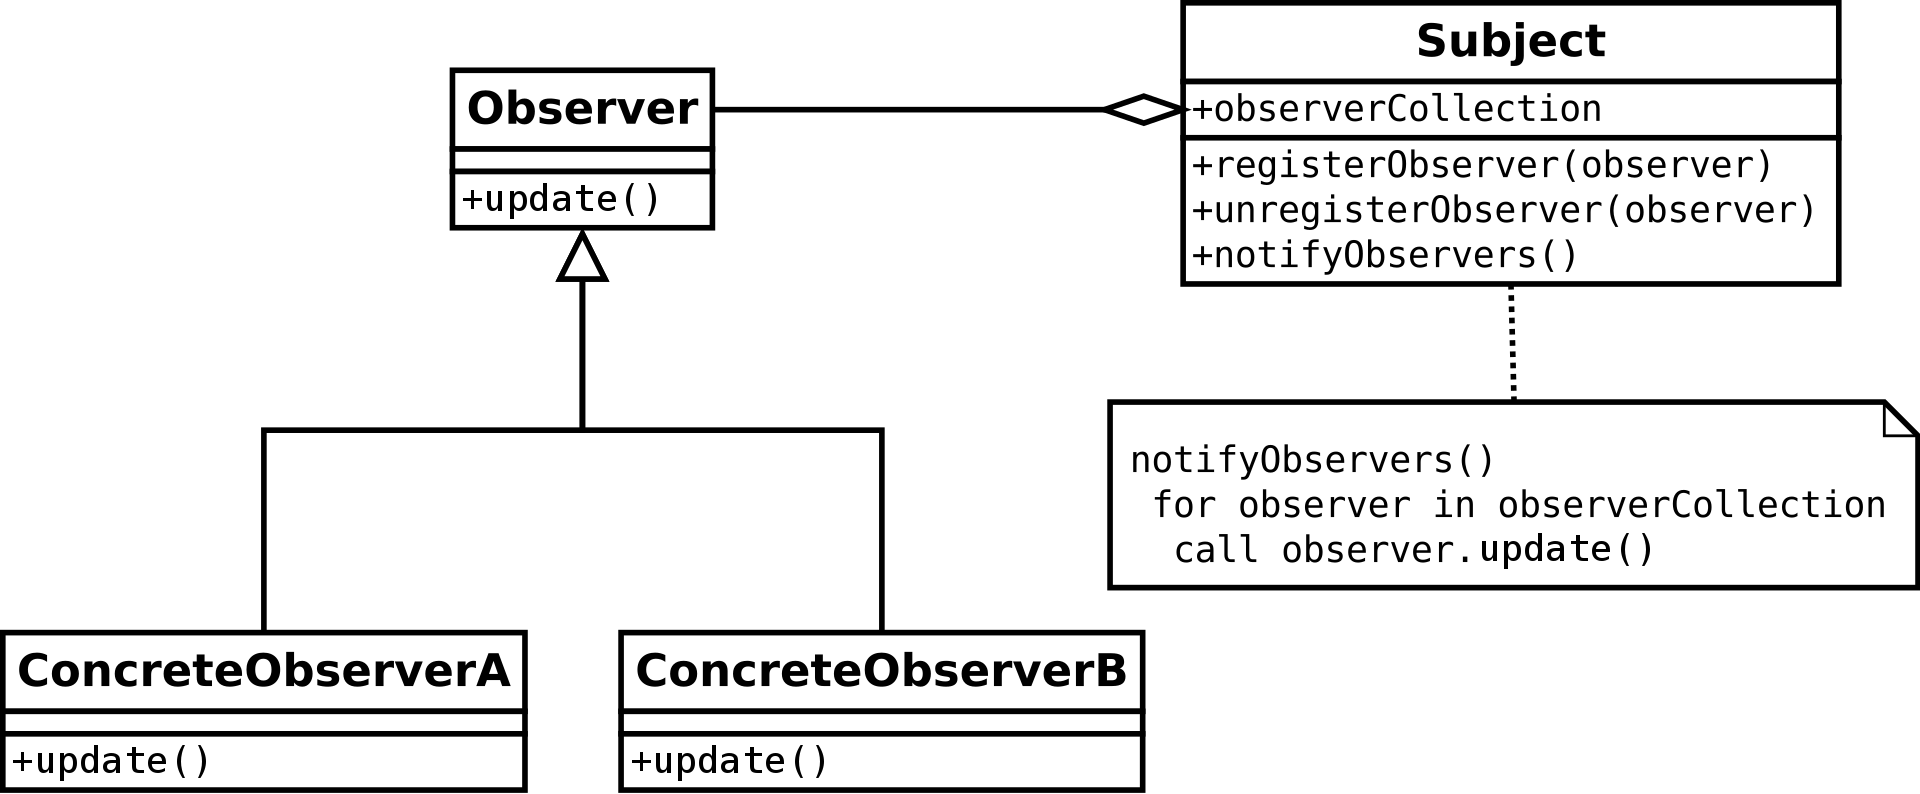
\includegraphics[width=1\textwidth]{observerpattern.png}
	\end{frame}
	
	
	\begin{frame}
		\frametitle{LiveData}
		\begin{quote}\textbf{LiveData} is an \textbf{observable data holder} class. Unlike a regular observable, \textbf{LiveData is lifecycle-aware}, meaning it respects the lifecycle of other app components, such as activities, fragments, or services. This awareness ensures \textbf{LiveData only updates} app component observers that are in an \textbf{active lifecycle} state\end{quote} developer.android.com \linebreak(official documentaion of android)
	\end{frame}
	

	\begin{frame}
	\frametitle{LifeCycle Awarenes}
	\begin{itemize}
	\item Observer almost everytime need an LifeCycle
	\item only exception when using "observeForever" method
	\item LifeCycles are provided by the Activity and/or Fragments 
	\item Observer only observe while the passed LifeCycle is (STARTED/RESUMED)
	\item Observer do not observe when the LifeCycle is PAUSED or in a dead state
	\end{itemize}
	Fazit: make sure, to have an lifecycle when you want to observe
	\end{frame}	
	
	\subsection[LiveData in Code]{LiveData in Code}
	\begin{frame}[fragile]
	\frametitle{Code example}
		\begin{block}{Create MutableLiveData}
		\begin{spverbatim}
			val liveData = MutableLiveData<String>().apply{
			value = "Hello World"
			}
		\end{spverbatim}
		Modify MutableLiveData with operations like \textit{postValue()} or \textit{setValue()} 		(which only can be called from the main-thread)
		\end{block}
		\begin{block}{Create LiveData}
		\begin{spverbatim}
			@Query("SELECT * FROM PERSON ORDER BY NAME")
			LiveData<List<Person>> loadAllPersons();
		\end{spverbatim}
	\end{block}
	\end{frame}
	
	\begin{frame}[fragile]
	\frametitle{Code example}
		\begin{block}{Create LiveData using MutableLiveData}
		\begin{spverbatim}
			private val privateLiveData = MutableLiveData<String>().apply{
			value = "Hello World"
			}
			val publicLiveData : LiveData<String> = privateLiveData
			
			fun changeString(string : String){
			privateLiveData.postValue(string)
			}
		\end{spverbatim}
	\end{block}
	\end{frame}
	
	\begin{frame}[fragile]
	\frametitle{Code example}
		\begin{block}{Observing LiveData with Observer object}
			\begin{spverbatim}
			val nameObserver = Observer<String> { newName ->
        	nameTextView.text = newName
    		}
			publicLiveData.observe(lifeCycleOwner, nameObserver)
		\end{spverbatim}
	\end{block}
	\begin{block}{Observing LiveData with Lambda}
		\begin{spverbatim}
			// not observed
			val name = repository.publicLiveData
			// make line above observing indirectly
			val nameLetters = name.observe(
			lifeCycleOwner,
			Observer{it.toCharArray().asList()}
			)
		\end{spverbatim}
	\end{block}
	\end{frame}
	
	\subsection[LiveData in Databinding]{LiveData in Databinding}
	\begin{frame}
	\frametitle{Observing Livedata + Databinding }
	\textbf{Fragment}
	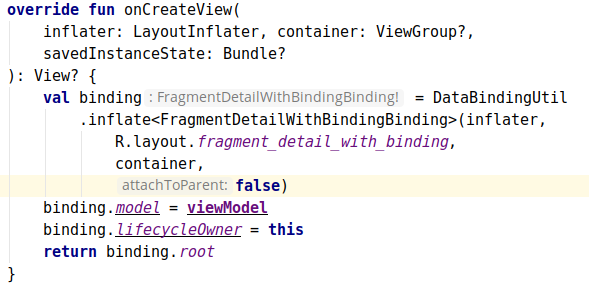
\includegraphics[width=1\textwidth]{DataBindingInFragment.png}
	\textbf{XML}
	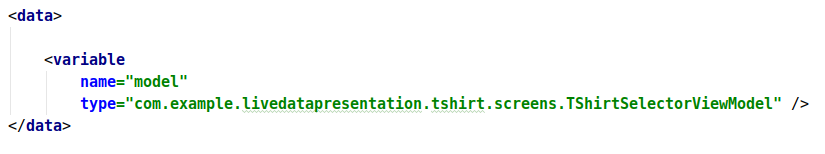
\includegraphics[width=1\textwidth]{DataBindingInXML.png}
	\end{frame}
	
	\begin{frame}	
	\frametitle{Observing Livedata + Databinding}
	\textbf{XML}
	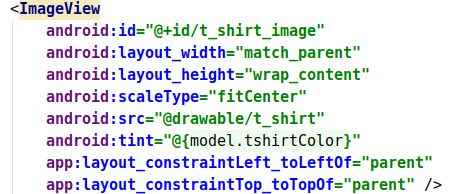
\includegraphics[width=1\textwidth]{DataBindingInImageView.png}
	\end{frame}
	
	\begin{frame}	
	\frametitle{Observing Livedata + Databinding}
	\textbf{XML}
	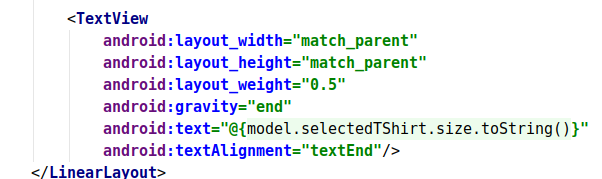
\includegraphics[width=1\textwidth]{DataBindingInTextView.png}
	\end{frame}
	
	\section[App Structure]{build LiveData into the Architecture}
	\subsection[General]{General App Structure}
	\begin{frame}
		\frametitle{Overall Structure of Android Apps}
		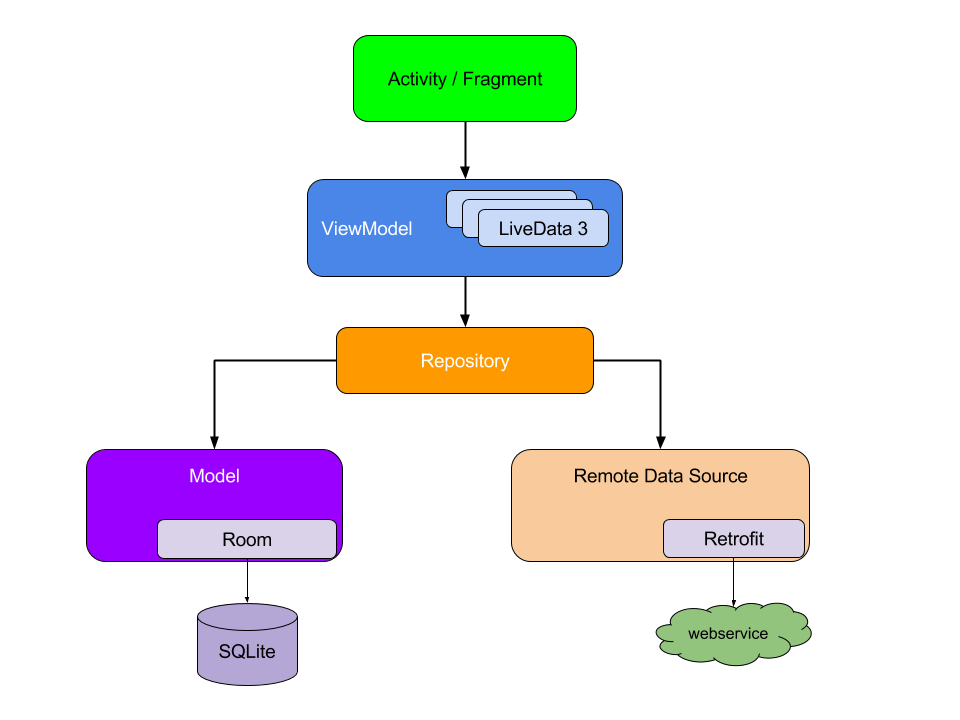
\includegraphics[width=1\textwidth]{architecture.png}
	\end{frame}
	
	\begin{frame}
		\frametitle{Overall Structure of Android Apps}
		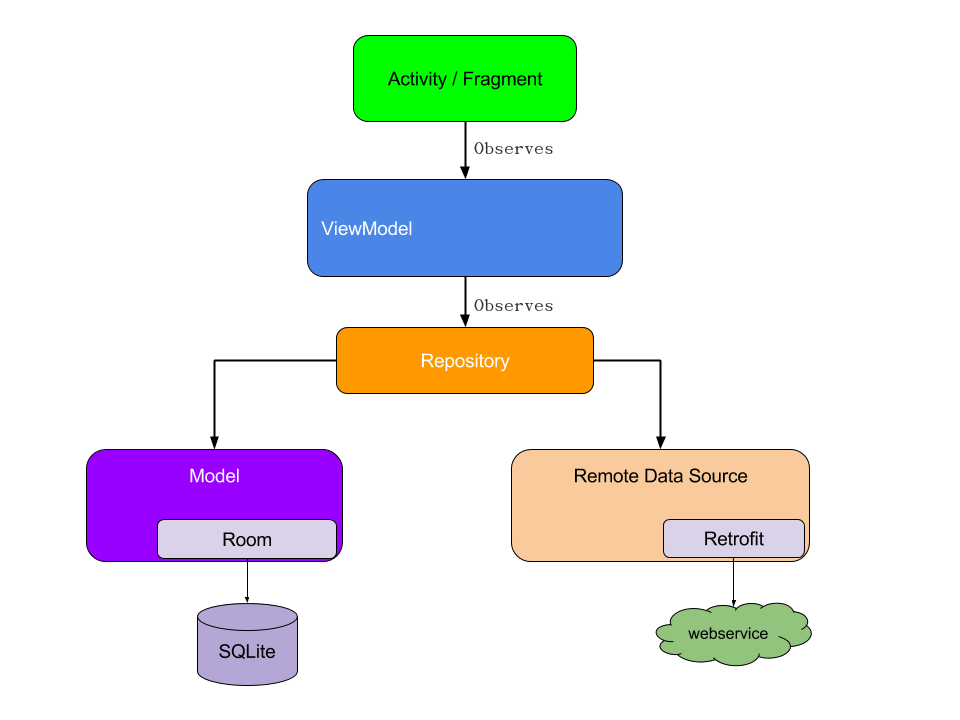
\includegraphics[width=1\textwidth]{architecture_observes.png}
	\end{frame}
	
	\subsection[My App]{My small T-Shirt App}
	\begin{frame}
		\frametitle{T-Shirt App Fragments}
		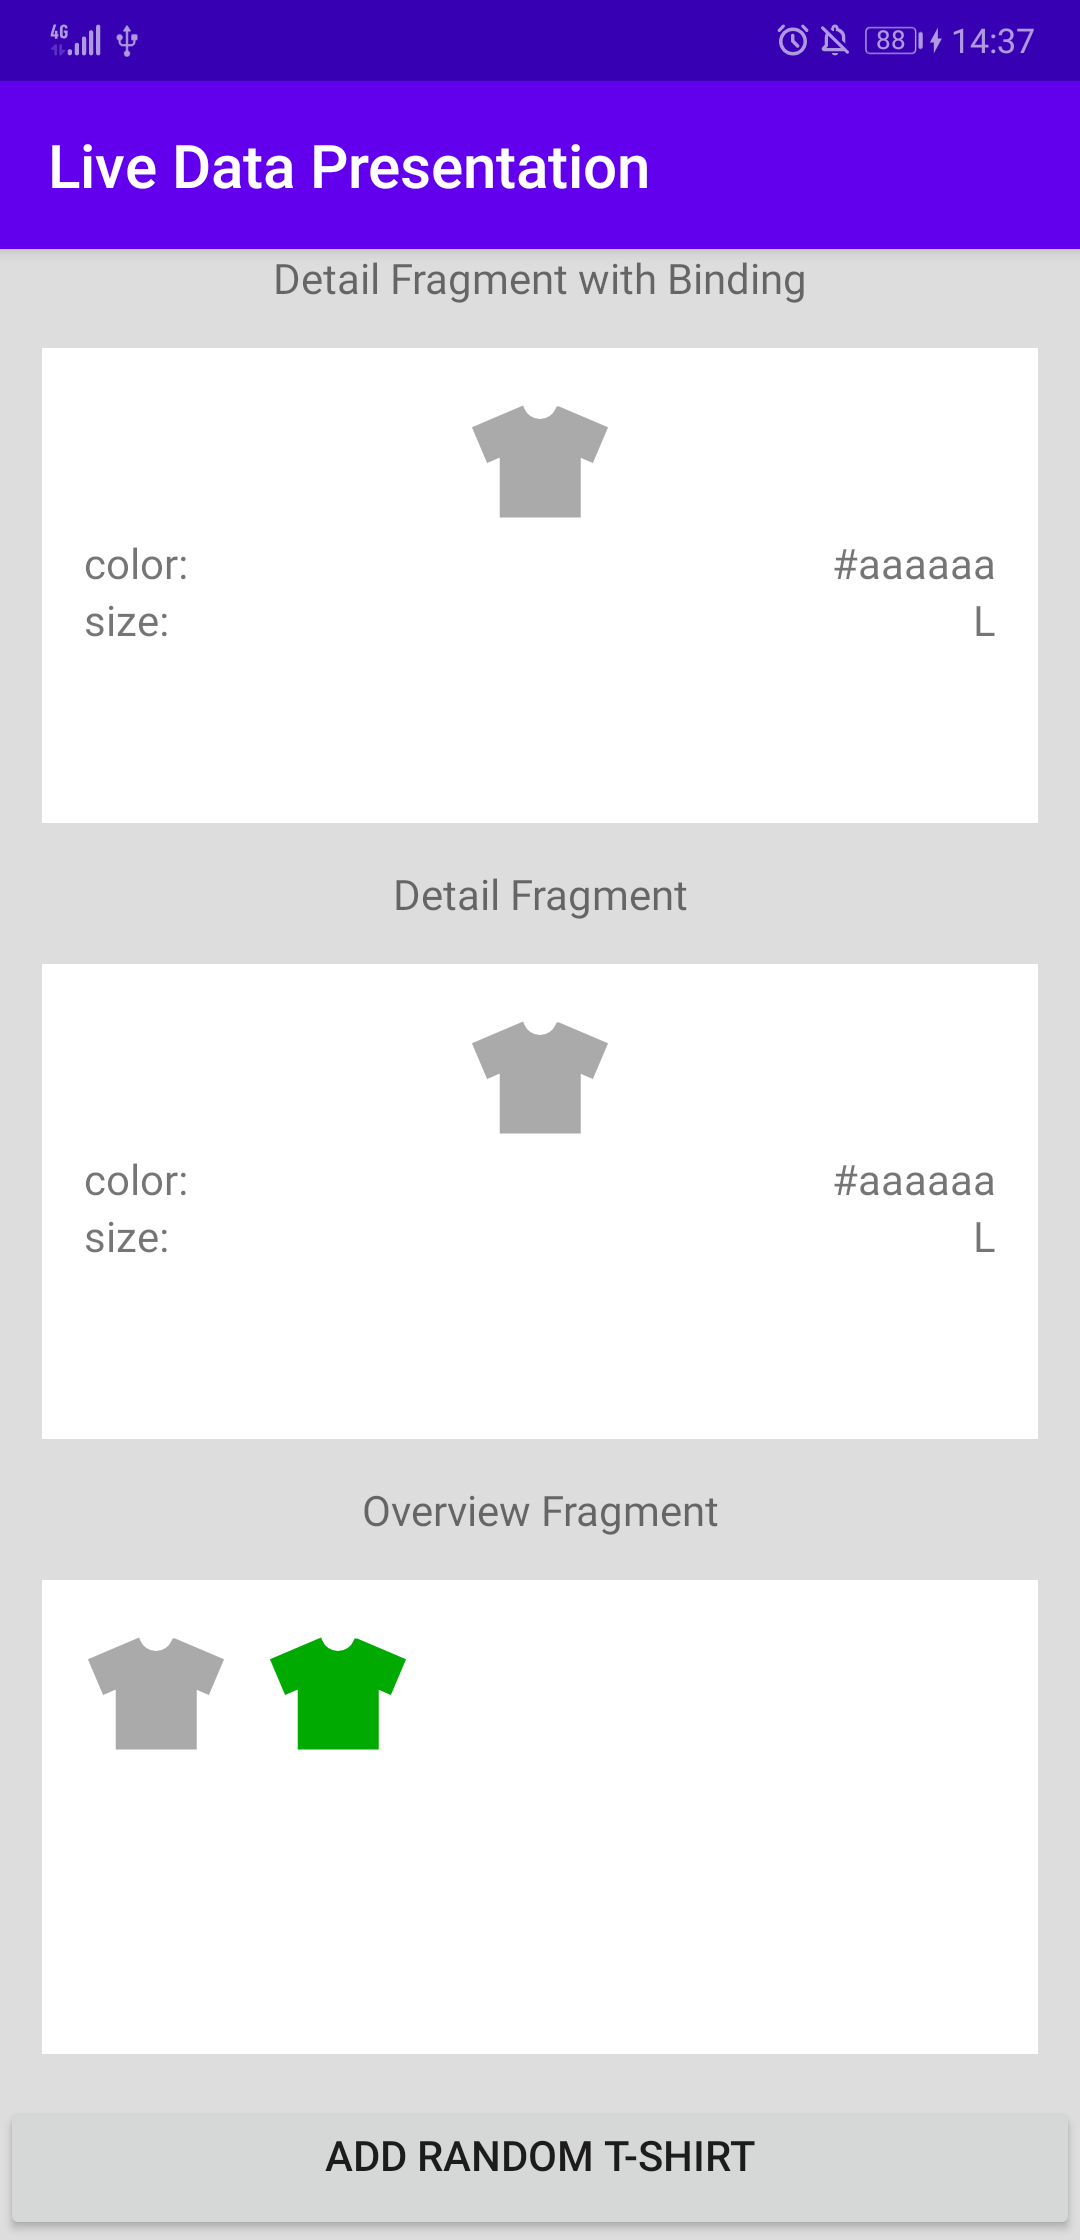
\includegraphics[width=0.3\textwidth]{screenshot_basic.png}
		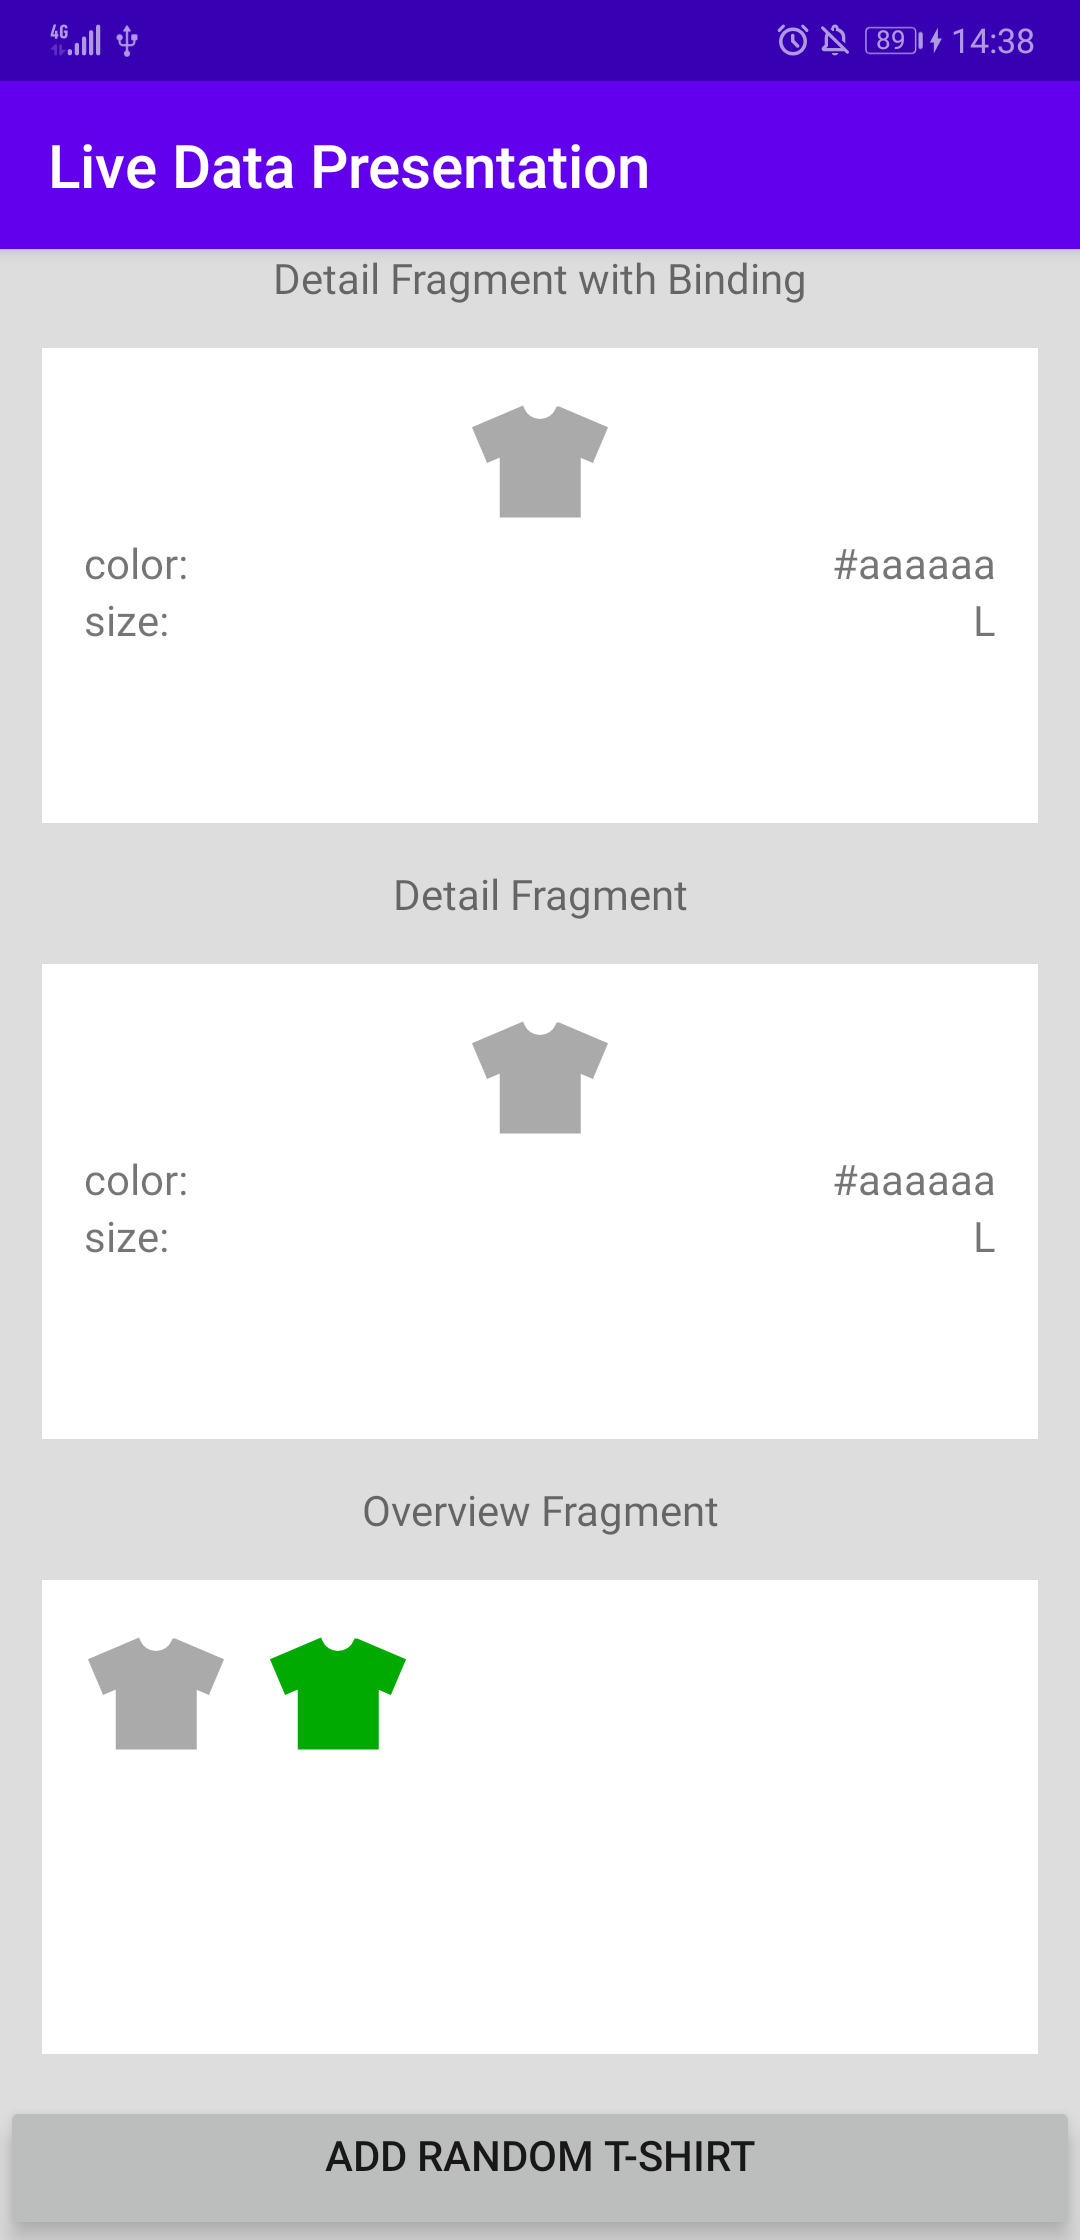
\includegraphics[width=0.3\textwidth]{screenshot_pressed.png}
		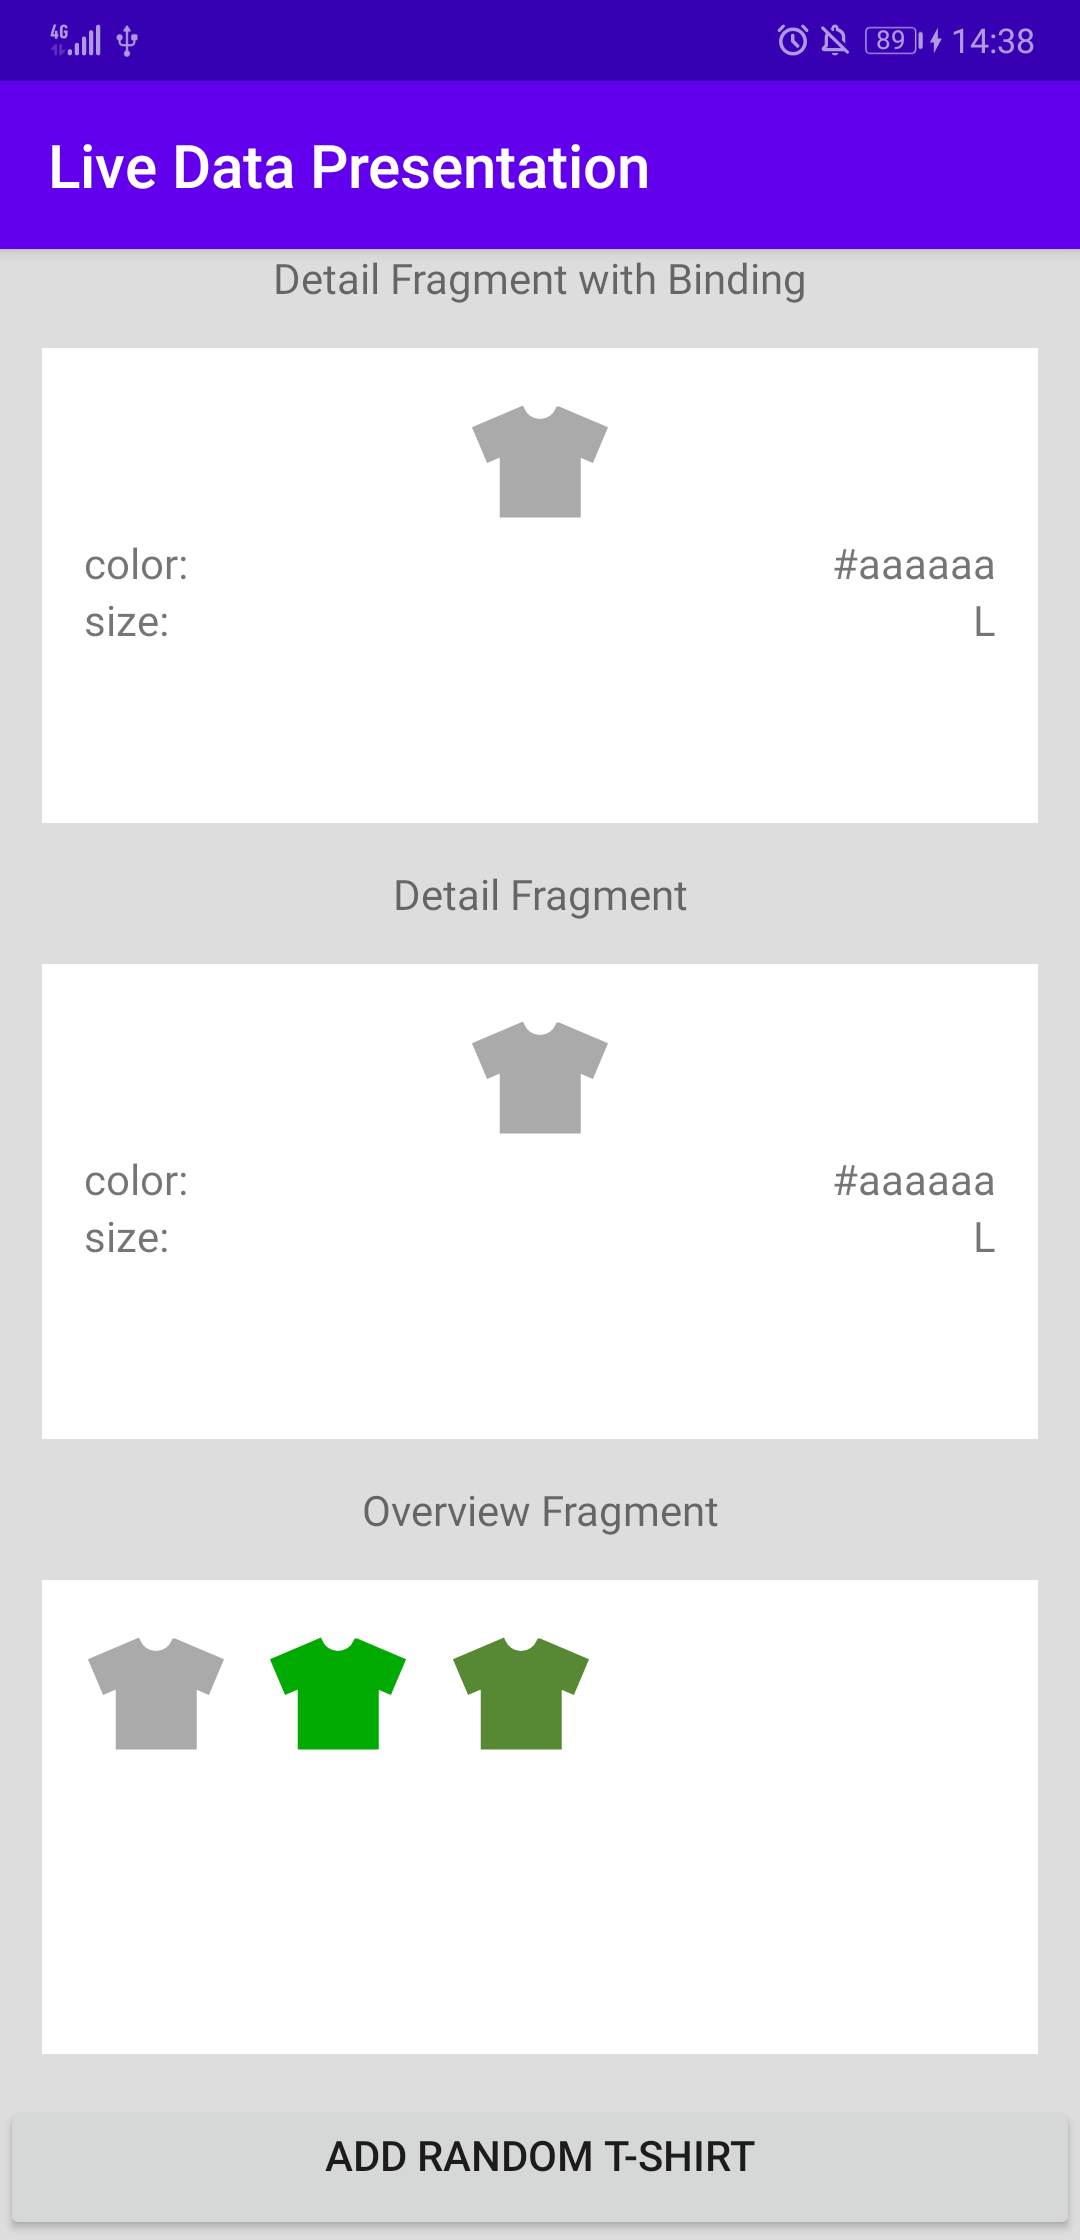
\includegraphics[width=0.3\textwidth]{screenshot_released.png}		
	\end{frame}
	
	\begin{frame}
	\frametitle{T-Shirt App Fragments}
	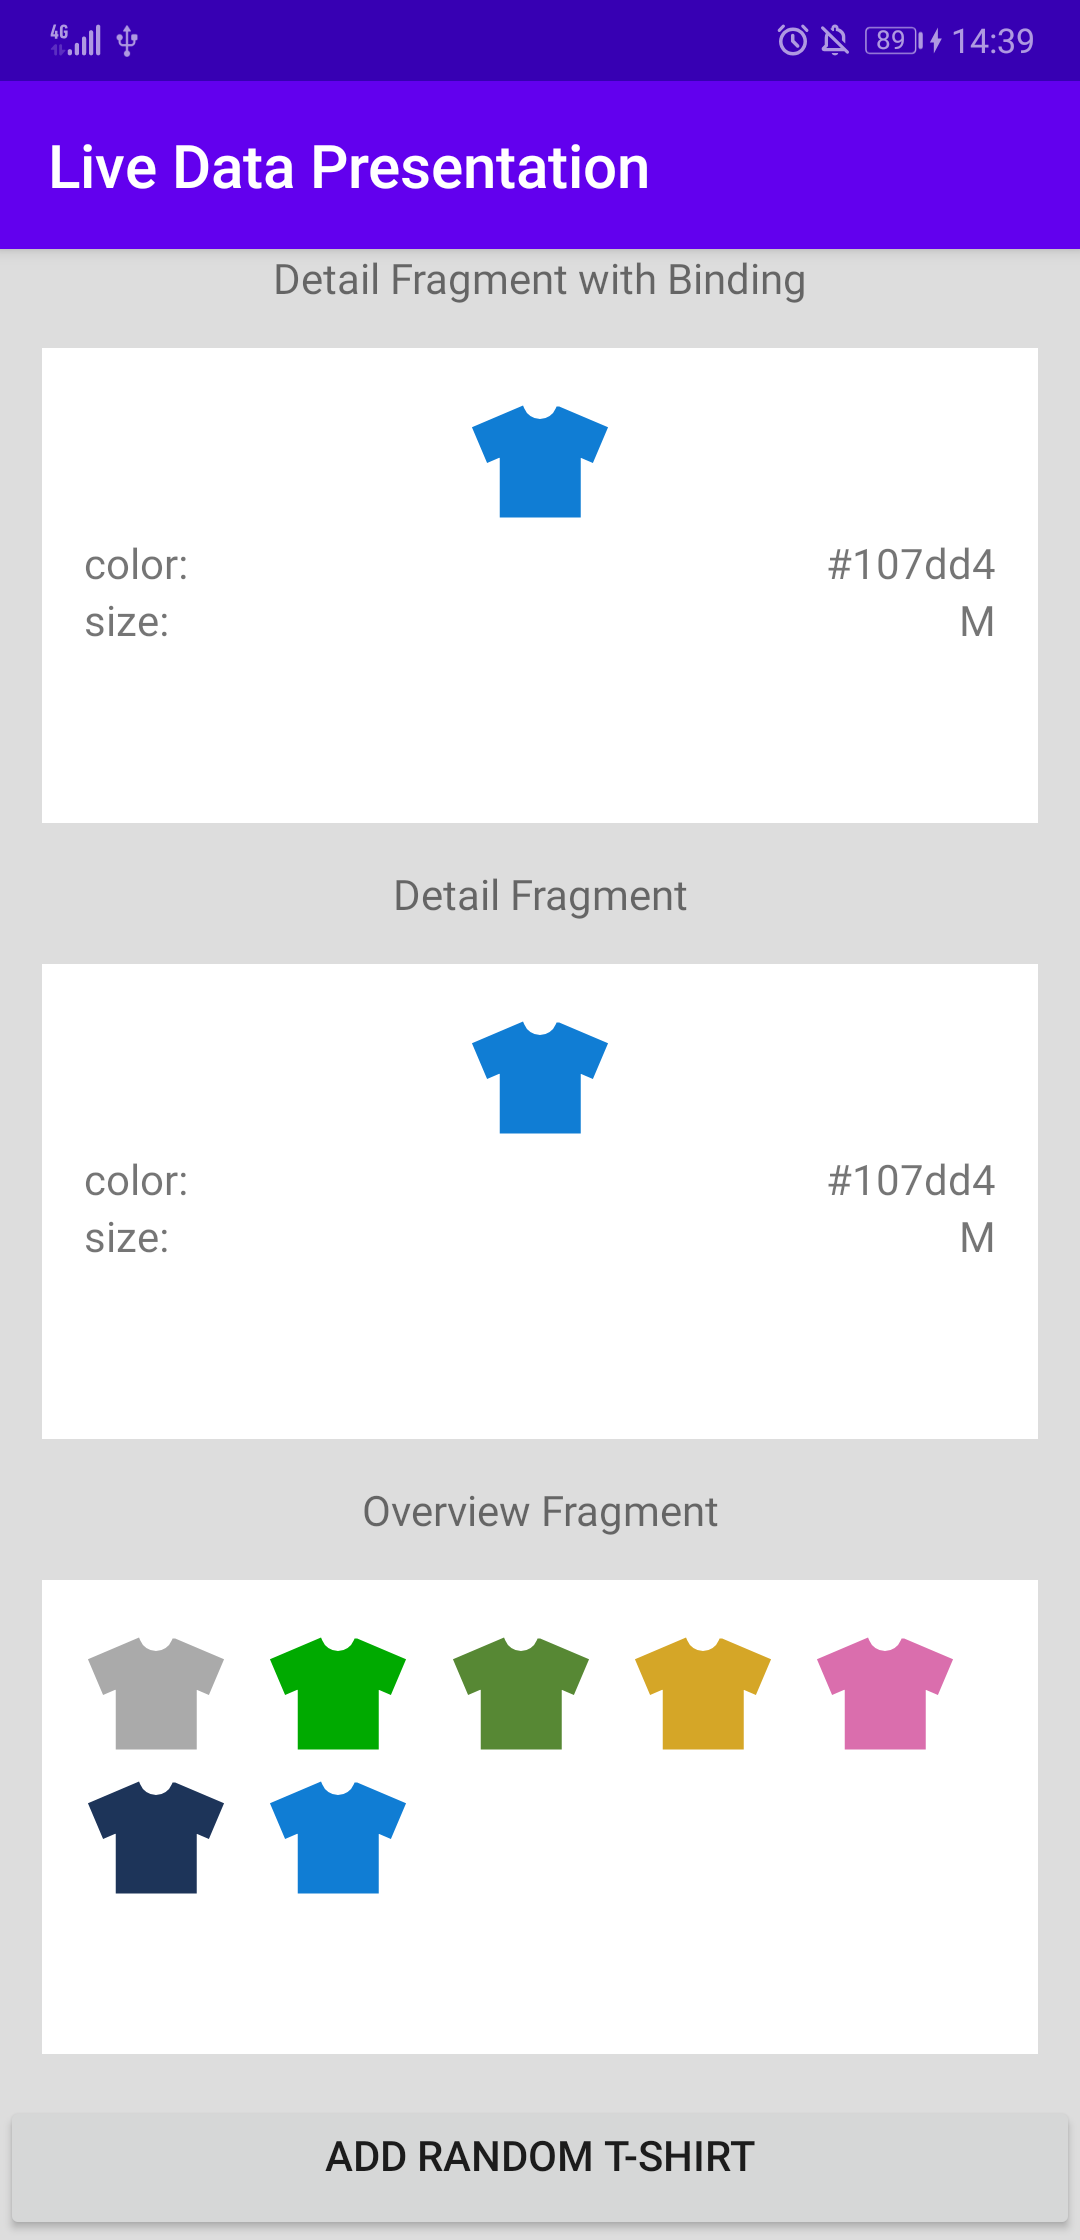
\includegraphics[width=0.3\textwidth]{multiple_shirts_blue.png}
	\hspace*{0.3\textwidth}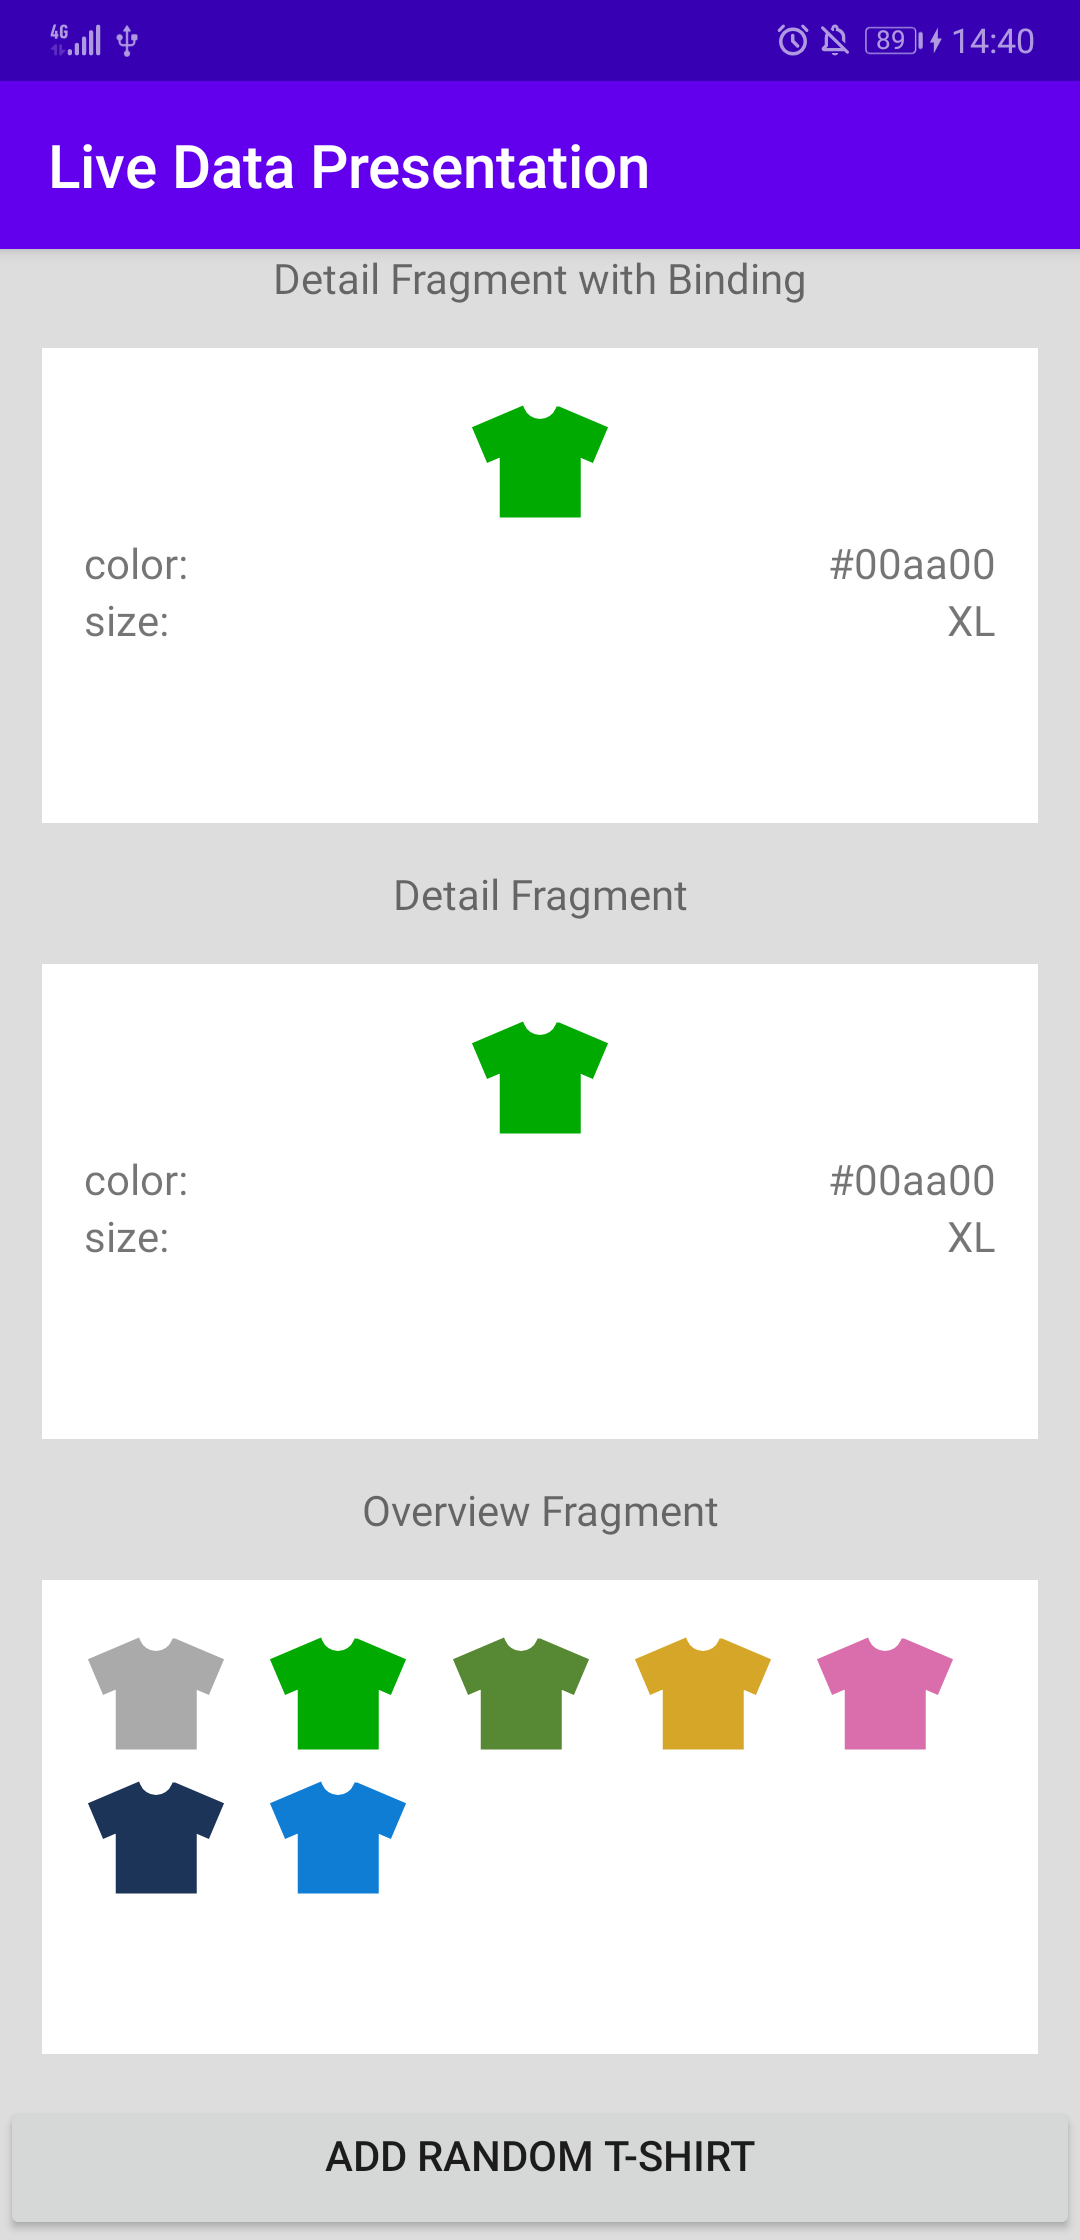
\includegraphics[width=0.3\textwidth]{multiple_shirts_green.png}
	\end{frame}
	\subsection[Implementation]{LiveData in the T-Shirt App}
	\begin{frame}
		\frametitle{LiveData in the T-Shirt App}
		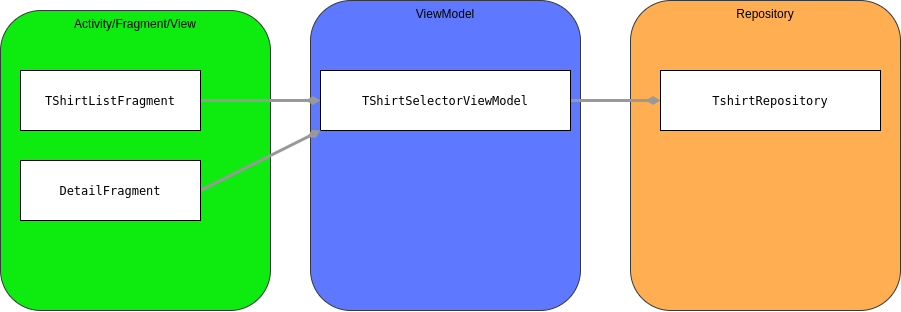
\includegraphics[width=1\textwidth]{TshirtArchitectureOverview.png}
	\end{frame}
	
	\begin{frame}
		\frametitle{LiveData in the T-Shirt App}
		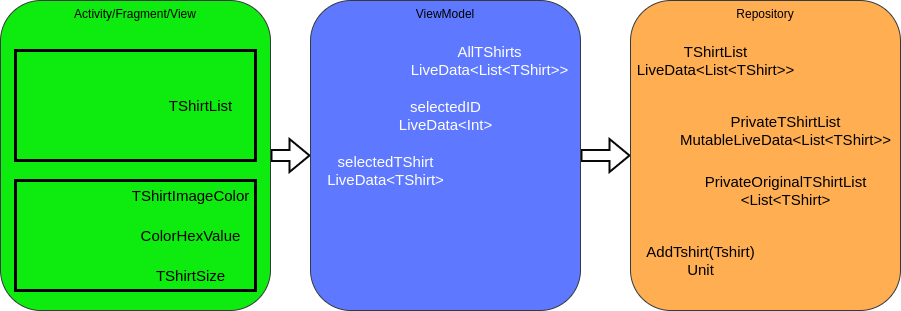
\includegraphics[width=1\textwidth]{TShirtAppDetailView.png}
	\end{frame}
	
	\section[Summary]{Summary}
	\begin{frame}
		\frametitle{Summary}
		\begin{itemize}
		\item check LifeCycle
		
		no observation when LifeCycle is Paused
		\item pass lifecycle to binding
		\item check if LiveData is observed
		
		not observed LiveData does not change
		\item check value is in proper Type in xml
		
		android:text = "@\{viewmodel.number\}"
		
			$\neq$
		
		android:text = "@\{viewmodel.number.toString()\}" 
		\item check Livedata is not Mutable acidently
		
		\end{itemize}
	\end{frame}
	
	\begin{frame}
		\frametitle{more information}
		\begin{itemize}
			\item udemy.com/course/android-jetpack/
			\item medium.com/androiddevelopers/viewmodels-and-livedata-patterns-antipatterns-21efaef74a54
		\end{itemize}
		developer.android.com:
		\begin{itemize}
			\item /topic/libraries/architecture/livedata
			\item /reference/androidx/lifecycle/Transformations
			\item /jetpack/docs/guide
		\end{itemize}
	\end{frame}
	
		\begin{frame}
		\frametitle{Questions?}
		\textbf{Thank you for your attention}
		\linebreak
		Feel free to ask me anything about
		\begin{itemize}
		\item LiveData
		\item Android General
		\item work in the internship
		\end{itemize}
		Repo:\\
		github.com/Tosaa/mobile-application-presentation
		
	\end{frame}
	
\end{document}
